\documentclass[11pt]{article}
\usepackage[utf8]{inputenc}
\usepackage{amsmath}
\usepackage{amssymb}
\usepackage{graphicx}
\usepackage{hyperref}
\usepackage[parfill]{parskip}
\let\oldemptyset\emptyset
\let\emptyset\varnothing


\title{\textbf{Esssentials of Applied Data Analysis\\
				IPSA-USP Summer School 2017}\newline\\
				Special Probability Distributions}

\author{Leonardo Sangali Barone\\ \href{leonardo.barone@usp.br}{leonardo.barone@usp.br}}
\date{jan/17}

\begin{document}

\maketitle

\section*{Special Probability Distributions}

	\subsection*{Probability Distributions}
	We have seen yesterday what random variables (both discrete and continuous) probability functions and probability distributions are. (Can you define all of theses concepts?)\\
	
	Today, we start by looking at some known probability distributions. Some distributions, as we will see, are derived from a known random proccess, hence, we can precisely describe them matematically. These distributions are called special probability distributions or probability models and they can be normally found in our data.

	\subsection*{Probability Distributions - most well-known}
	We are going to cover only a few distributions:\\

	Discrete: 
	\begin{itemize}
		\item Uniform
		\item Bernoulli
		\item Binomial
	\end{itemize}
	
	Continuous:
	\begin{itemize}
		\item Uniform
		\item Normal
		\item Exponential
		\item Chi-square (gamma)
		\item F
		\item t-student
	\end{itemize}
		
	\subsection*{Discrete Probability Distributions - Uniform}
	The uniform distribution is the simple case of probability model (for discrete and continuous variables). Distributions of the class have in common the fact that every value of the random variable has the same probability of occuring.\\
	
	In the discrete case, $P(X=x_i) = 1/k$, where k is the number of possible outcomes for the variable.\\

	In the continuous case, the probability function is $f(x_i) = 1/b-a$, and $[a,b]$ is the interval that contains all possible outcomes of the variable.

	\subsection*{Discrete Probability Distributions - Uniform}
	The expected value of a uniform variable is:\\

	Discrete:
	\[E[X] = \frac{1}{k} \sum\limits_{i=1}^k x_i\]

	Continuous:
	\[E[X] = \frac{(a+b)}{2} \]

	The variance of a uniform variable is:\\
	
	Discrete:
	\[E[X] = \frac{1}{k} (\sum\limits_{i=1}^k x_i^2-(\sum\limits_{i=1}^k x_i)^2/k\]

	Continuous:
	\[E[X] = \frac{(a+b)^2}{12} \]

	\subsection*{Discrete Probability Distributions - Bernoulli}
	Imagine any expetiment that has a probability of success $P(X=1) = p$ and a probability of failure $P(X=0) = 1-p = q$. An experiment like this is a Bernoulli experiment and it generates a distribution.\\

		The expected value of a Bernoulli variable is:
		\[E[X] = p\]

		and the variance is:
		\[Var[X]=p-p^2= p*(1-p) = p*q\]

	\subsection*{Discrete Probability Distributions - Binomial}
	
	Now, instead of executiong the Bernoulli experiment only once, let's do the experiment $n$ times and count the number of successes.\\

	Let's do it on stata.\\

	\begin{verbatim}
	clear
	set obs 1000
	gen x = rbinomial(100, .5)
	hist x, discrete
	\end{verbatim}

	The expected value of a Binomial variable is:
		\[E[X] = n*p\]
		
	and the variance is:
		\[Var[X]=n*(p-p^2)= n*p*(1-p) = n*p*q\]

	Call $x$ the number of successes and n the number of Bernoulli experiments. The probability of each $x$ can be obtained by:
		\[P(X=x)\binom{n}{x} * p^x * (1-p)^{n-x}\]
		
		(Note: For the beaty of this, read the chapter teen of Alex Bellos book.)	

	For example, let's toss a coin 5 times. What is the distribution of the number of heads (success)?\newline\\
		\begin{tabular}{|c|c|}
\hline
	Number of heads $(x)$ & $P(X=x)$\\
\hline
0 & $\binom{5}{0} * (0.5)^0 * (0.5)^{5-0}$\\
1 & $\binom{5}{1} * (0.5)^1 * (0.5)^{5-1}$\\
2 & $\binom{5}{2} * (0.5)^2 * (0.5)^{5-2}$\\
3 & $\binom{5}{3} * (0.5)^3 * (0.5)^{5-3}$\\
4 & $\binom{5}{4} * (0.5)^4 * (0.5)^{5-4}$\\
5 & $\binom{5}{5} * (0.5)^5 * (0.5)^{5-5}$\\
\hline
\end{tabular}


\begin{figure}[htp]
\centering
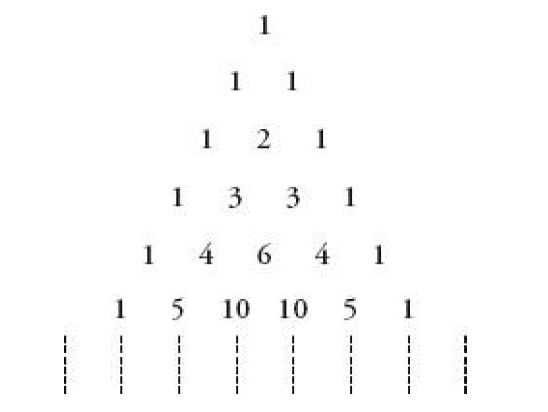
\includegraphics[scale=0.5]{pascal.png}
\caption{Pascal triangle}
\label{}
\end{figure}

\begin{figure}[htp]
\centering
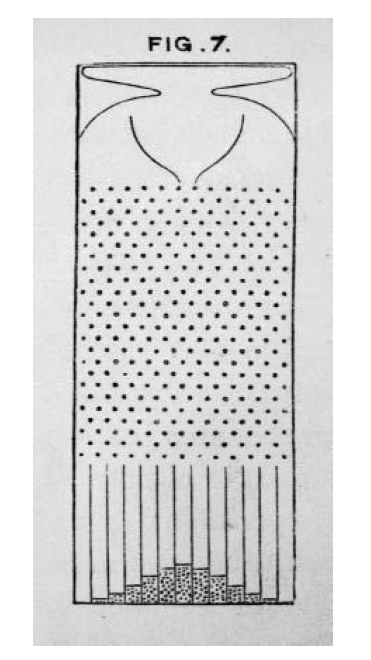
\includegraphics[scale=0.3]{game.png}
\caption{The Quincux}
\label{}
\end{figure}

\begin{figure}[htp]
\centering
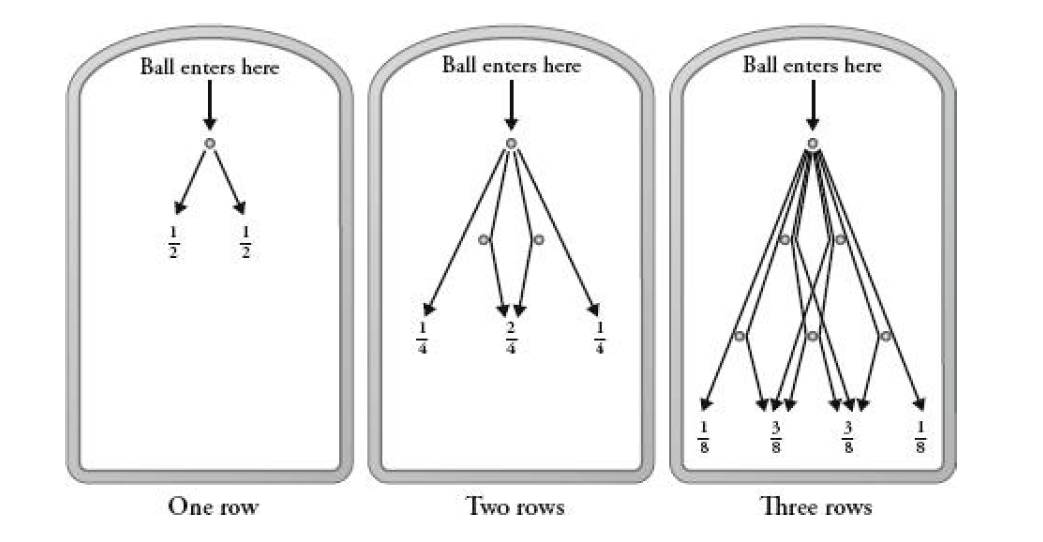
\includegraphics[scale=0.3]{game2.png}
\caption{The Quincux}
\label{}
\end{figure}


We will see that when we draw a great number of times from the binomial distribution, which is discrete, we tend to approximate from another important distribution, the normal distribution.

	\begin{verbatim}
	clear
	set obs 1000000
	gen x = rbinomial(100,.5)
	hist x, discrete normal
	\end{verbatim}

	\subsection*{Discrete Probability Distributions - Normal distribuiton}

The normal distribuition is of great importance for statistics. A lot of phenomenon in daily life, nature of social sciences tend to be normally distributed.


A normal distribution has two parameters: $\mu$ and $\sigma$. The probability function of a normal distribution is:
\[f(x|\mu,\sigma)=\frac{1}{\sigma \sqrt{2\pi}}e^{\frac{(x-\mu)^2}{2\sigma^2}}\]
where $E[X]=\mu$ and $Var[X]=\sigma^2$.

\begin{figure}[htp]
\centering
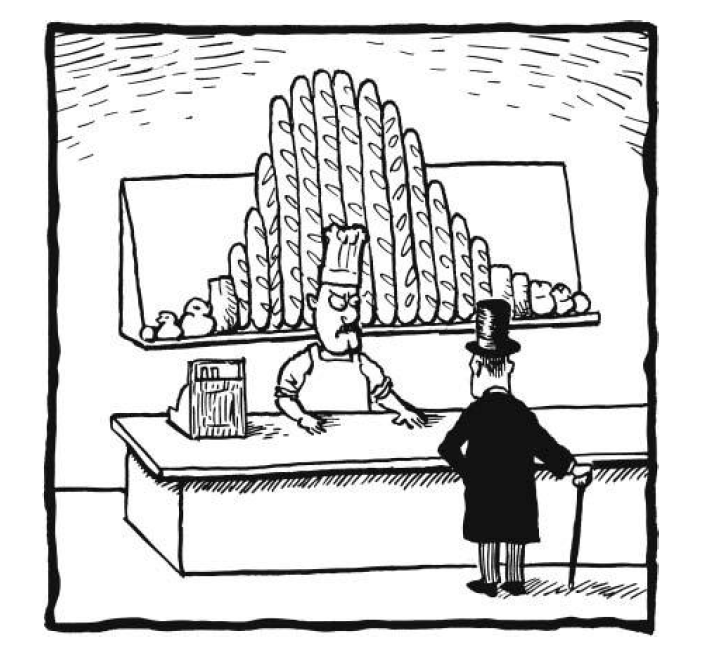
\includegraphics[scale=0.4]{pao.png}
\caption{Normal Distribution}
\label{}
\end{figure}


\end{document}
